\documentclass[
    12pt, % Schriftgröße
    DIV10,
    ngerman, % für Umlaute, Silbentrennung etc.
    a4paper, % Papierformat
    oneside, % einseitiges Dokument
    titlepage, % es wird eine Titelseite verwendet
    parskip=half, % Abstand zwischen Absätzen (halbe Zeile)
    headings=normal, % Größe der Überschriften verkleinern
    listof=totoc, % Verzeichnisse im Inhaltsverzeichnis aufführen
    bibliography=totoc, % Literaturverzeichnis im Inhaltsverzeichnis aufführen
    index=totoc, % Index im Inhaltsverzeichnis aufführen
    captions=tableheading, % Beschriftung von Tabellen unterhalb ausgeben
    final % Status des Dokuments (final/draft)
]{scrartcl}

% Pakete

% Schrift ----------------------------------------------------------------------
\usepackage{lmodern} % bessere Fonts

% Paket für Kopfzeilen und Fußzeilen
\usepackage[
    automark, % Kapitelangaben in Kopfzeile automatisch erstellen
    headsepline, % Trennlinie unter Kopfzeile
    ilines % Trennlinie linksbündig ausrichten
]{scrpage2}

% Anpassung an Landessprache
\usepackage[ngerman]{babel}

% Umlaute ----------------------------------------------------------------------
%   Umlaute/Sonderzeichen wie äöüß direkt im Quelltext verwenden (CodePage).
%   Erlaubt automatische Trennung von Worten mit Umlauten.
% ------------------------------------------------------------------------------
\usepackage[utf8]{inputenc}
\usepackage[T1]{fontenc}
\usepackage{textcomp} % Euro-Zeichen etc.

\usepackage[babel,german=quotes]{csquotes}

% Bei Änderungen müssen die *.aux und *.bbl Dateien manuell gelöscht werden
% Sonst kommt es zu einem Fehler bei der Erstellung
%\usepackage[round, sort, comma, numbers]{natbib}
%\usepackage[round, numbers]{natbib}
%\bibliographystyle{abbrvdin}
%

\usepackage{scrhack}

\usepackage[citestyle=alphabetic,bibstyle=alphabetic,backend=biber]{biblatex}
\bibliography{Bibliographie}
\DefineBibliographyStrings{german}{
  bibliography = {Literaturverzeichnis},
}
\setlength\bibitemsep{8pt}

\usepackage{xpatch}
\xpretobibmacro{author}{\mkbibbold\bgroup}{}{}
\xapptobibmacro{author}{\egroup}{}{}
\xpretobibmacro{editor}{\mkbibbold\bgroup}{}{}
\xapptobibmacro{editor}{\egroup}{}{}
\xpretobibmacro{editor+others}{\mkbibbold\bgroup}{}{}
\xapptobibmacro{editor+others}{\egroup}{}{}
\xpretobibmacro{bbx:editor}{\mkbibbold\bgroup}{}{}
\xapptobibmacro{bbx:editor}{\egroup}{}{}

% Grafiken ---------------------------------------------------------------------
% Einbinden von JPG-Grafiken ermöglichen
\usepackage[dvips,final]{graphicx}
\graphicspath{{Bilder/}}

% Paket zur Verwendung zusätzlicher Positionsbefehle
\usepackage{float}

% Befehle aus AMSTeX für mathematische Symbole z. B. \boldsymbol \mathbb --------
\usepackage{amsmath,amsfonts}

% Einfache Definition der Zeilenabstände und Seitenränder etc. -----------------
\usepackage{setspace}
\usepackage{geometry}

% zum Umfließen von Bildern ----------------------------------------------------
\usepackage{floatflt}

% Farbdefinitionen
\usepackage{xcolor} 
\definecolor{hellgelb}{rgb}{1,1,0.9}
\definecolor{colKeys}{rgb}{0,0,1}
\definecolor{colIdentifier}{rgb}{0,0,0}
\definecolor{colComments}{rgb}{1,0,0}
\definecolor{colString}{rgb}{0,0.5,0}
\definecolor{whgreen}{RGB}{113,177,41}
\definecolor{dvBlue}{RGB}{0,85,160}

% URL verlinken, lange URLs umbrechen etc. -------------------------------------
\usepackage{url}

% PDF-Optionen -----------------------------------------------------------------
\usepackage[
    bookmarks,
    bookmarksopen=true,
    colorlinks=true,
% diese Farbdefinitionen zeichnen Links im PDF farblich aus
    linkcolor=dvBlue, % einfache interne Verkn�pfungen
    anchorcolor=black,% Ankertext
    citecolor=dvBlue, % Verweise auf Literaturverzeichniseintr�ge im Text
    filecolor=magenta, % Verkn�pfungen, die lokale Dateien �ffnen
    menucolor=dvBlue, % Acrobat-Men�punkte
    urlcolor=dvBlue, 
% diese Farbdefinitionen sollten für den Druck verwendet werden (alles schwarz)
%    linkcolor=black, % einfache interne Verkn�pfungen
%    anchorcolor=black, % Ankertext
%    citecolor=black, % Verweise auf Literaturverzeichniseintr�ge im Text
%    filecolor=black, % Verkn�pfungen, die lokale Dateien �ffnen
%    menucolor=black, % Acrobat-Men�punkte
%    urlcolor=black, 
    %backref, % Inkompatibel mit BibLateX
    plainpages=false, % zur korrekten Erstellung der Bookmarks
    pdfpagelabels, % zur korrekten Erstellung der Bookmarks
    hypertexnames=false, % zur korrekten Erstellung der Bookmarks
    linktocpage % Seitenzahlen anstatt Text im Inhaltsverzeichnis verlinken
]{hyperref}

% fortlaufendes Durchnummerieren der Fußnoten ----------------------------------
\usepackage{chngcntr}
%\counterwithout{footnote}{chapter}

% Formatierung von Listen ändern -----------------------------------------------
\usepackage{paralist} % itemize, enumerate

% bei der Definition eigener Befehle benötigt
\usepackage{ifthen} % Vielleicht nicht nötig

% definiert u.a. die Befehle \ und \listoftodos
\usepackage{todonotes}
\reversemarginpar

% sorgt dafür, dass Leerzeichen hinter parameterlosen Makros nicht als Makroendezeichen interpretiert werden
\usepackage{xspace}

\usepackage{tabularx} % Tabellenspalten mit variabler Breite
\usepackage{wrapfig}  % Schriftumflossene Bilder


% Seitenstil

% Zeilenabstand 1,5 Zeilen
\onehalfspacing

% Seitenränder
% bottom is 20 + X, weil Footer nicht berücksichtigt wird
\geometry{paper=a4paper,left=30mm,right=20mm,top=20mm, bottom=38mm, footskip=8mm}

% Kopf- und Fußzeilen ----------------------------------------------------------
% Kopf- und Fußzeile auch auf Kapitelanfangsseiten
%\renewcommand*{\chapterpagestyle}{scrheadings} 
% Schriftform der Kopfzeile
%\renewcommand{\headfont}{\normalfont}

% Kopfzeile
\ihead{\headmark} % links
\chead{}
%\ohead{\includegraphics[scale=0.1]{Bilder/DJLogo.png}} % rechts
\setlength{\headheight}{20mm} % Höhe der Kopfzeile
% Kopfzeile über den Text hinaus verbreitern
%\setheadwidth[0pt]{textwithmarginpar} 
\setheadsepline[text]{0.4pt} % Trennlinie unter Kopfzeile

% Fußzeile
%\ifoot{} % links
\cfoot{} % mitte
\ofoot{\pagemark} % rechts
%\setfootsepline[text]{0.4pt} % Trennlinie unter Kopfzeile



% Schusterjungen und Hurenkinder vermeiden
%\clubpenalty = 10000
%\widowpenalty = 10000 
%\displaywidowpenalty = 10000

% Verringert den Abstand über den Überschriften
%\renewcommand*{\chapterheadstartvskip}{\vspace*{-\topskip}}

% Irgendwas mit Silbentrennung in MonoSpace (texttt)
\newcommand{\origttfamily}{}% sollte noch nicht definiert sein!
\let\origttfamily=\ttfamily % alte Definition von \ttfamily sichern
\renewcommand{\ttfamily}{\origttfamily \hyphenchar\font=`\-}


% Eigene Befehle und typographische Auszeichnungen für diese

\newcommand{\bs}{$\backslash$}

% einige Befehle zum Zitieren --------------------------------------------------
\newcommand{\Zitat}[2][\
empty]{\ifthenelse{\equal{#1}{\empty}}{\citep{#2}}{\citep[#1]{#2}}}

% zum Ausgeben von Autoren
\newcommand{\AutorName}[1]{\textsc{#1}}
\newcommand{\Autor}[1]{\AutorName{\citeauthor{#1}}}

% Produktnamen
\newcommand{\produkt}[1]{\textbf{#1}}

\newcommand{\code}[1]{\texttt{#1}}

% zum Einbinden von Programmcode -----------------------------------------------
\usepackage{listings}
\usepackage{xcolor}
\usepackage{textcomp}
\lstset{
    float=hbp,
    basicstyle=\fontsize{10}{9}\ttfamily\color{black},
    identifierstyle=\color{colIdentifier},
    keywordstyle=\color{colKeys},
    stringstyle=\color{colString},
    commentstyle=\color{colComments},
    %columns=flexible,
    tabsize=2,
    frame=single,
    extendedchars=true,
    showspaces=false,
    showstringspaces=false,
    numbers=left,
    numberstyle=\ttfamily\small,
    numbersep=5pt,
    breaklines=true,
    backgroundcolor=\color{hellgelb},
    breakautoindent=true
}

\lstset{literate=
  {á}{{\'a}}1 {é}{{\'e}}1 {í}{{\'i}}1 {ó}{{\'o}}1 {ú}{{\'u}}1
  {Á}{{\'A}}1 {É}{{\'E}}1 {Í}{{\'I}}1 {Ó}{{\'O}}1 {Ú}{{\'U}}1
  {à}{{\`a}}1 {è}{{\'e}}1 {ì}{{\`i}}1 {ò}{{\`o}}1 {ù}{{\`u}}1
  {À}{{\`A}}1 {È}{{\'E}}1 {Ì}{{\`I}}1 {Ò}{{\`O}}1 {Ù}{{\`U}}1
  {ä}{{\"a}}1 {ë}{{\"e}}1 {ï}{{\"i}}1 {ö}{{\"o}}1 {ü}{{\"u}}1
  {Ä}{{\"A}}1 {Ë}{{\"E}}1 {Ï}{{\"I}}1 {Ö}{{\"O}}1 {Ü}{{\"U}}1
  {â}{{\^a}}1 {ê}{{\^e}}1 {î}{{\^i}}1 {ô}{{\^o}}1 {û}{{\^u}}1
  {Â}{{\^A}}1 {Ê}{{\^E}}1 {Î}{{\^I}}1 {Ô}{{\^O}}1 {Û}{{\^U}}1
  {œ}{{\oe}}1 {Œ}{{\OE}}1 {æ}{{\ae}}1 {Æ}{{\AE}}1 {ß}{{\ss}}1 {Δ}{{$\Delta$}}1
  {ç}{{\c c}}1 {Ç}{{\c C}}1 {ø}{{\o}}1 {å}{{\r a}}1 {Å}{{\r A}}1
  {€}{{\EUR}}1 {£}{{\pounds}}1
}

\usepackage{microtype}

\renewcommand*{\dictumwidth}{.41\textwidth}
\renewcommand*{\dictumrule}{}
\renewcommand*{\dictumauthorformat}[1]{--- #1}
\setkomafont{dictumauthor}{%
\scshape
}

\definecolor{bluekeywords}{rgb}{0,0,1}
\definecolor{greencomments}{rgb}{0,0.5,0}
\definecolor{redstrings}{rgb}{0.64,0.08,0.08}
\definecolor{xmlcomments}{rgb}{0.5,0.5,0.5}
\definecolor{types}{rgb}{0.17,0.57,0.68}

\lstdefinestyle{csharp}
{
    language=[Sharp]C,
    captionpos=b,
    %numbers=left, %Nummerierung
    %numberstyle=\tiny, % kleine Zeilennummern
    showspaces=false,
    showtabs=false,
    breaklines=true,
    showstringspaces=false,
    breakatwhitespace=true,
    escapeinside={(*@}{@*)},
    commentstyle=\color{greencomments},
    morekeywords={partial, var, value, get, set},
    keywordstyle=\color{bluekeywords},
    stringstyle=\color{redstrings},
    basicstyle=\ttfamily\small,
}

\lstdefinestyle{hive}
{
    language=SQL,
    captionpos=b,
    %numbers=left, %Nummerierung
    %numberstyle=\tiny, % kleine Zeilennummern
    showspaces=false,
    showtabs=false,
    breaklines=true,
    showstringspaces=false,
    breakatwhitespace=true,
    escapeinside={(*@}{@*)},
    commentstyle=\color{greencomments},
    morekeywords={bigint, double, decimal, char, string, row, format, lines, location, DELIMITED, FIELDS, TERMINATED, STORED, TEXTFILE,
    	OVERWRITE, DIRECTORY},
    keywordstyle=\color{bluekeywords},
    stringstyle=\color{redstrings},
    basicstyle=\ttfamily\small,
}

\lstdefinestyle{xml}
{
    language=XML,
    captionpos=b,
    %numbers=left, %Nummerierung
    %numberstyle=\tiny, % kleine Zeilennummern
    showspaces=false,
    showtabs=false,
    breaklines=true,
    showstringspaces=false,
    breakatwhitespace=true,
    escapeinside={(*@}{@*)},
    commentstyle=\color{greencomments},
    morekeywords={encoding},
    keywordstyle=\color{bluekeywords},
    stringstyle=\color{redstrings},
    basicstyle=\ttfamily\small,
}

\colorlet{punct}{red!60!black}
\definecolor{background}{HTML}{EEEEEE}
\definecolor{delim}{RGB}{20,105,176}
\colorlet{numb}{magenta!60!black}

\lstdefinelanguage{json}{
    basicstyle=\normalfont\ttfamily,
    numbers=left,
    numberstyle=\scriptsize,
    stepnumber=1,
    numbersep=8pt,
    showstringspaces=false,
    breaklines=true,
    frame=single,
    literate=
     *{0}{{{\color{numb}0}}}{1}
      {1}{{{\color{numb}1}}}{1}
      {2}{{{\color{numb}2}}}{1}
      {3}{{{\color{numb}3}}}{1}
      {4}{{{\color{numb}4}}}{1}
      {5}{{{\color{numb}5}}}{1}
      {6}{{{\color{numb}6}}}{1}
      {7}{{{\color{numb}7}}}{1}
      {8}{{{\color{numb}8}}}{1}
      {9}{{{\color{numb}9}}}{1}
      {:}{{{\color{punct}{:}}}}{1}
      {,}{{{\color{punct}{,}}}}{1}
      {\{}{{{\color{delim}{\{}}}}{1}
      {\}}{{{\color{delim}{\}}}}}{1}
      {[}{{{\color{delim}{[}}}}{1}
      {]}{{{\color{delim}{]}}}}{1},
}

%\usepackage{caption} 
%\captionsetup[table]{skip=100pt}
% Bindet die Literaturdaten ein!
\bibliography{Bibliographie}
\begin{document}

%Startstruktur
\setcounter{secnumdepth}{3}
\setcounter{tocdepth}{2}

\pagestyle{empty}
\thispagestyle{plain}
\begin{titlepage}

\begin{center}


\includegraphics[scale=0.7]{Deckblatt/WH_Logo.jpg}

\vspace{2cm}

\Huge{\textbf{Urlaubsgenehmigung}}\\[1.5ex]
\Large{\textbf{Projektdokumentation}}
\rule{\textwidth}{0.4pt}\\[3.0ex]

\large{\textbf{im Masterstudiengang Verteilte Systeme}}\\[3.0ex]

\normalsize
\begin{tabular}{ll}\\
	vorgelegt von: 
	& \quad Dennis Miller, \\[1.2ex]
	& \quad Christian Schlütter\\[1.2ex]
	& \quad \\[1.2ex]
	Modul:  & \quad Business Process Management (BPM) \\[1.2ex]
	Gutachter:  & \quad Prof. Dr. Jürgen Priemer \\[1.2ex]
	Abgabetermin:  & \quad \today\\[1.2ex]
\end{tabular}

\end{center}

\end{titlepage}


\tableofcontents
\setcounter{page}{1}

\pagestyle{scrheadings}

\newpage


\section{Aufgabenstellung}
Unsere Aufgabenstellung ist es einen Workflow zur Urlaubsgenehmigung in einem Unternehmen nachzubilden. Dabei sollen bestimmte Geschäftsregeln (s. Abschnitt \ref{Geschäftsregeln}) auf eine beispielhafte Personalhierarchie (s. Abschnitt \ref{Personalhierarchie}) abgebildet werden.

Ziel unserer Aufgabe ist die Entwicklung einer prototypischen Anwendung, die den Urlaubsgenehmigungsprozess in einem BPMN-Diagramm zeigt und eine Interaktion mit dem Endanwender ermöglicht.

\subsection{Geschäftsregeln}
\label{Geschäftsregeln}

Für den Urlaubsgenehmigungsprozess in unserem Beispielunternehmen gelten die folgenden Regeln:
\begin{enumerate}
	\item Reicht ein Mitarbeiter einen Urlaubsantrag ein, so ist dieser bei 20 Werktagen oder weniger
	immer an den direkten Vorgesetzten weiter zu leiten und durch diesen zu genehmigen oder
	abzulehnen. Hat der direkte Vorgesetzte nach drei Tagen noch nicht über den Urlaubsantrag
	entschieden (z.B. weil er nicht da ist), wird der Urlaubsantrag eine Ebene höher geleitet.
	\item Wird ein Urlaub von mehr als 20 Werktagen beantragt, so muss dieser zusätzlich vom Leiter der
	Personalabteilung genehmigt werden.
	\item Wenn ein Urlaubsantrag abgelehnt wurde, ist der Mitarbeiter in Kenntnis zu setzen.
	\item Wenn ein Urlaubsantrag genehmigt wurde, ist er sofort an zuständigen Sachbearbeiter in der
	Personalabteilung weiter zu leiten. Diese prüft, ob noch genügend Urlaubstage zur Verfügung
	stehen. Ist dies nicht der Fall und es handelt sich nicht um Sonderurlaub (siehe unten), wird der
	Urlaubsantrag an den Vorgesetzen zurückgegeben und kann nicht genehmigt werden.
	\item Sonderurlaub kann gewährt werden bei Umzug (max. 1 Tag), Geburt- oder Todesfall (max. 2
	Tage) oder als Bonus (max. 3 Tage). Sonderurlaub wird nicht auf die normalen Urlaubstage
	angerechnet.
	\item Sonderurlaubsanträge für Umzug und Geburts- oder Todesfälle sind immer automatisch zu
	genehmigen. Ein Bonus-Urlaub ist durch Vorgesetzten und den Leiter der Personalabteilung zu
	genehmigen.
	\item Über den Urlaub eines Vorstandsmitglieds entscheidet der Vorstandsvorsitzende. Urlaubsanträge
	des Vorstandsvorsitzenden werden dem stellvertretenden Vorstandsvorsitzenden vorgelegt.
	Urlaube von Vorstandsmitgliedern von weniger als 5 Tagen müssen nicht genehmigt (aber
	natürlich in der Personalabteilung vermerkt werden. Bei Vorstandsmitgliedern wird ein
	Überziehen des zur Verfügung stehenden Urlaubs um maximal 3 Tage geduldet.
	\item Normale Mitarbeiter erhalten 30 Tage Urlaub pro Jahr, Mitglieder des Vorstands 25 Tage.
\end{enumerate}

\subsection{Personalhierarchie}
\label{Personalhierarchie}

Im Beispielunternehmen ist die folgende Personalhierarchie gegeben:
\begin{figure}[H]
\centering
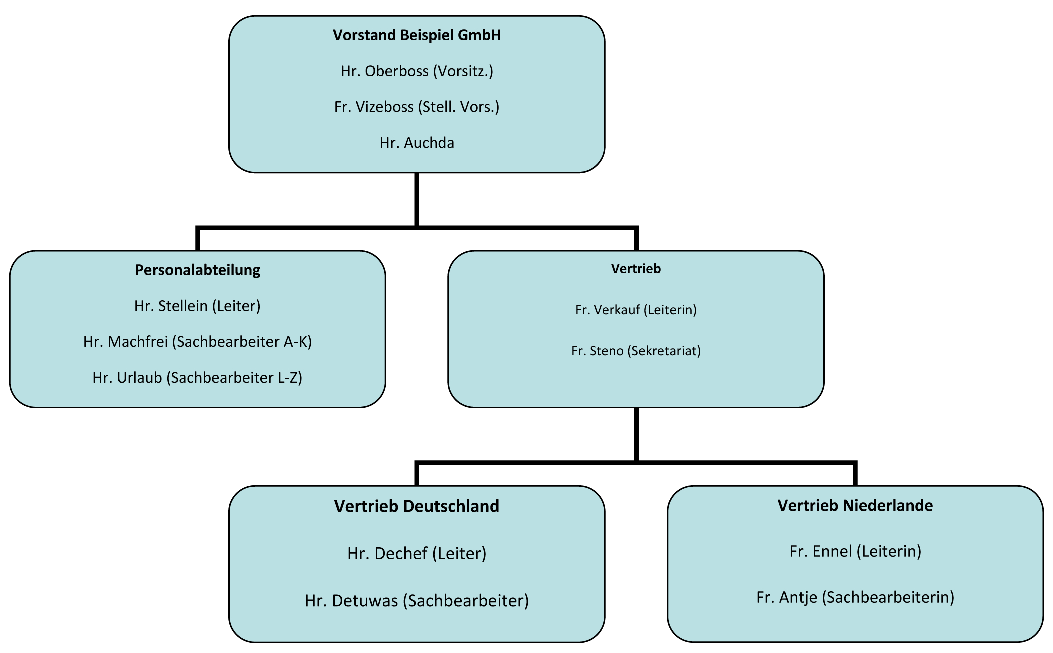
\includegraphics[width=1.0\linewidth]{Bilder/Hierarchie}
\caption[]{Personalhierarchie unseres Beispielunternehmens\footnotemark}
\label{fig:Hierarchie}
\end{figure}
\footnotetext{Quelle: Aufgabe Urlaubsgenehmigung jBPM.pdf}

In der Personalhierarchie gibt es einige erwähnenswerte Besonderheiten. In der Personalabteilung gibt es zwei Sachbearbeiter mit unterschiedlichen Zuständigkeiten. Herr Machfrei ist für die Mitarbeiter, deren Nachname mit einem Buchstaben zwischen A und K beginnen, zuständig. Herr Urlaub bearbeitet die Übrigen, deren Nachnamen mit L bis Z beginnen.\\
Des Weiteren ist der Vorgesetzte im abteilungsübergreifenden Falle immer Leiter der entsprechend höheren Abteilung. Gleiches gilt für den stellvertretenden Vorgesetzten. Für die Vorstandsebene ergibt sich die Besonderheit, dass der "`Vorgesetzte"' des Oberbosses der Vizeboss ist.
Der stellvertretende Vorgesetzte des Oberbosses ist somit wiederum der Oberboss selbst. Gleiches gilt für den Vizeboss, dessen stellvertretender Vorgesetzter er selbst ist.



\section{Werkzeuge}
\subsection{KIE Workbench}
\subsection{Eclipse JBPM Modeler 2}
\section{Implementierung}
In diesem Kapitel wollen wir auf die Implementierung unseres Prototypen eingehen.


\subsection{Vorstellung des Ablaufs}
Zunächst beschreiben wir dazu den grundsätzlichen Ablauf des Prozesses anhand einer Skizze:
\begin{figure}[H]
\centering
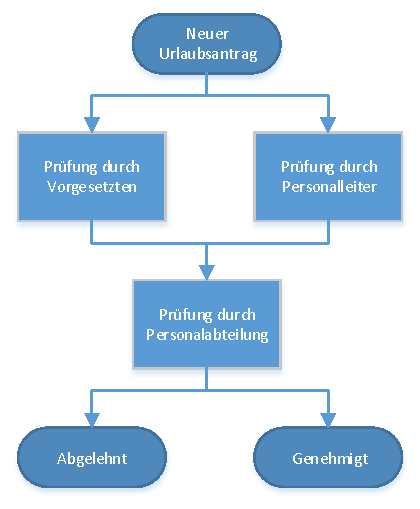
\includegraphics[width=0.5\linewidth]{Bilder/Workflow}
\caption{Skizze des Prozessablaufs}
\label{fig:Workflow}
\end{figure}

Hat ein Mitarbeiter einen Urlaubsantrag ausgefüllt startet ein neuer Urlaubsgenehmigungsprozess. Der Antrag muss an verschiedenen Stellen geprüft werden. In unserem Beispielunternehmen muss der Urlaubsantrag durch den Vorgesetzten und ggf. den Leiter der Personalabteilung genehmigt werden. Da die Reihenfolge hierbei keine Rolle spielt, können die beiden Schritte parallel ausgeführt werden. Abschließend prüft die Personalabteilung, ob der Mitarbeiter noch über genügend freie Urlaubstage verfügt und genehmigt bzw. verweigert den Antrag.	
	
	
\subsection{Systemübersicht}
Abbildung \ref{fig:Komponenten} stellt eine Übersicht unseres Systems dar. Um einen neuen Urlaubsgenehmigungsprozess starten zu können, müssen zunächst die erforderlichen Daten wie Name, Anzahl der Tage und Urlaubstyp vom Mitarbeiter eingegeben werden. Diese Daten werden im Urlaubsantragsobjekt Application\footnote{Mit Application ist hier der Antrag und nicht die Anwendung gemeint.}, welches über die Schnittstelle UserInterface angelegt wird, gespeichert.

\begin{figure}[H]
\centering
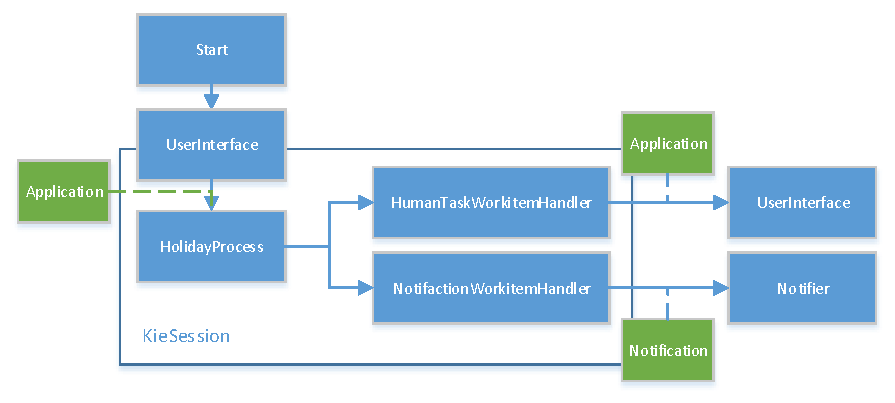
\includegraphics[width=0.93\linewidth]{Bilder/Komponenten}
\caption{Eine Übersicht der beteiligten Komponenten}
\label{fig:Komponenten}
\end{figure}

Nach Eingabe der Daten, wird eine neue KieSession erzeugt und ein neuer HolidayProcess gestartet. Dieser benötigt zur Abarbeitung der Workflow-Schritte insgesamt zwei WorkItemHandler. Der HumanTaskWorkItemHandler realisiert die Interaktion mit dem Endanwender und benötigt dazu die Schnittstelle UserInterface. Dabei werden die eingegebenen Daten jeweils in dem Datenobjekt Application gespeichert. Der NotificationWorkItemHandler ist für die Benachrichtigung der Mitarbeiter zuständig und verwendet dazu die Schnittstelle Notifier. Daten, die für das Benachrichtigen von Mitarbeitern relevant sind, werden in dem Datenobjekt Notification gespeichert.

Das verwendete Datenmodell und die benötigten Schnittstellen werden in den folgenden Abschnitten näher beschrieben.

\subsubsection{Datenmodell}
Wie Abbildung \ref{fig:Datenmodell} zeigt, besteht unser Datenmodell insgesamt aus zwei Klassen:

\begin{figure}[H]
\centering
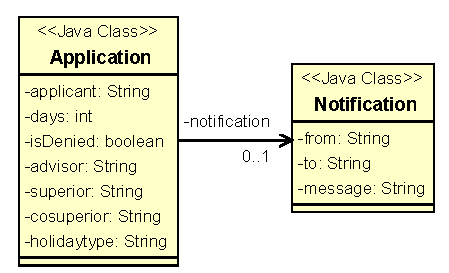
\includegraphics[width=0.5\linewidth]{Bilder/Datenmodell}
\caption{Datenmodell unserer Anwendung}
\label{fig:Datenmodell}
\end{figure}

In der Klasse Application werden alle Daten gespeichert, die für den Urlaubsantrag relevant sind. Neben dem Antragssteller (applicant) werden die Anzahl der Werktage (days) und der Typ des Urlaubs (holidaytype) gespeichert. Zudem ist der Vorgesetzte (superior), dessen Stellvertreter (cosuperior) und der zuständige Sachbearbeiter (advisor) hinterlegt. Außerdem speichern wir den Antragsstatus (isDenied) und eine dazugehörige Benachrichtigung (notification), die der Mitarbeiter abschließend erhält.

Die Klasse Notification repräsentiert die Daten für eine Benachrichtigung. Hier werden Absender, Empfänger und die Nachricht hinterlegt. 

\subsubsection{Schnittstellen}
\label{subsubsec:Schnittstellen}
\begin{figure}[H]
\centering
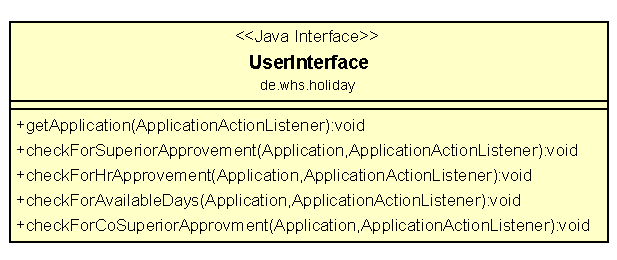
\includegraphics[width=0.7\linewidth]{Bilder/SchnittstelleUserInterface}
\caption{Die Schnittstelle UserInterface}
\label{fig:SchnittstelleUserInterface}
\end{figure}

Abbildung \ref{fig:SchnittstelleUserInterface} zeigt das UserInterface, worüber die Interaktion mit dem Endanwender realisiert wird. Die Funktionen repräsentieren dabei die verschiedenen Prozessschritte wie beispielsweise "`Genehmigung durch Vorgesetzten"' oder "`Prüfung ausreichend freier Urlaubstage"'. In unserer Anwendung gibt es zwei Implementierungen für das Interface: Eine Konsolenanwendung und eine GUI, die wir in Swing realisiert haben.

\begin{figure}[H]
\centering
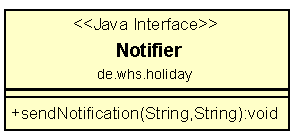
\includegraphics[width=0.35\linewidth]{Bilder/SchnittstelleNotifier}
\caption{Die Schnittstelle Notifier}
\label{fig:SchnittstelleNotifier}
\end{figure}

Zum Verschicken von Benachrichtigungen haben wir die Schnittstelle Notifier (s. Abbildung \ref{fig:SchnittstelleNotifier}) definiert. Für eine reale Unternehmensanwendung könnte man sich hier beispielsweise einen E-Mail-Dienst vorstellen. In unserer Anwendung haben wir die Benachrichtigung über eine Ausgabe in der Konsole bzw. Swing-GUI realisiert.

\begin{figure}[H]
\centering
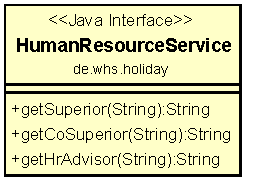
\includegraphics[width=0.3\linewidth]{Bilder/SchnittstelleHumanResourceService}
\caption{Die Schnittstelle HumanResourceService}
\label{fig:SchnittstelleHumanResourceService}
\end{figure}

Abbildung \ref{fig:SchnittstelleHumanResourceService} zeigt die Schnittstelle HumanResourceService, die es uns ermöglicht den Vorgesetzten, Stellvertreter und zuständigen Personalsachbearbeiter für den Antragssteller zu ermitteln. In der Realität könnte man hier beispielsweise das Active-Directory des Unternehmens oder eine gesonderte Anwendung einbinden. Für unseren Prototyp haben wir die Personalhierarchie unseres Beispielunternehmens, wie in Abbildung \ref{fig:Hierarchie} dargestellt, statisch hinterlegt.

\newpage
\subsection{Business Workflow}

\subsubsection{Benutzerdefinierte Aufgabe: Notification}
Um die Benachrichtigung des Mitarbeiters als einzelnen Prozessschritt in unserem BPMN-Diagramm zu realisieren, fehlte uns im Standard ein entsprechender Aufgabentyp. Daher haben wir diesen als benutzerdefinierte Aufgabe erstellt. Diese muss in einer Konfigurationsdatei definiert werden, auf die dann innerhalb der drools.rulebase.conf wie folgt verwiesen werden kann:
\begin{lstlisting}
drools.workDefinitions = HolidayWorkDefinitions.wid WorkDefinitions.conf
\end{lstlisting}

Die Definition für unsere benutzerdefinierte Aufgabe haben wir in der HolidayWorkDefinitions.wid wie folgt vorgenommen:

\begin{lstlisting}
import org.drools.core.process.core.datatype.impl.type.StringDataType;
[
  // the Notification work item
  [
    "name" : "Notification",
    "parameters" : [
      "Message" : new StringDataType(),
      "From" : new StringDataType(),
      "To" : new StringDataType()
    ],
    "displayName" : "Notification",
    "icon" : ""
  ]
]
\end{lstlisting}

Anschließend steht diese Aufgabe im Prozessdesigner als "`Custom Task"' zur Verfügung und kann innerhalb der Prozessdefinition wie die üblichen Elemente verwendet werden:

\vspace{20pt}
\begin{figure}[H]
\centering
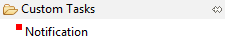
\includegraphics[width=0.4\linewidth]{Bilder/NotificationCustomTask}
\caption{Der CustomTask Notification}
\label{fig:NotificationCustomTask}
\end{figure}

Die definierten Felder finden sich in den Eigenschaften der benutzerdefinierten Aufgabe wieder und können entsprechend gefüllt werden:

\begin{figure}[H]
\centering
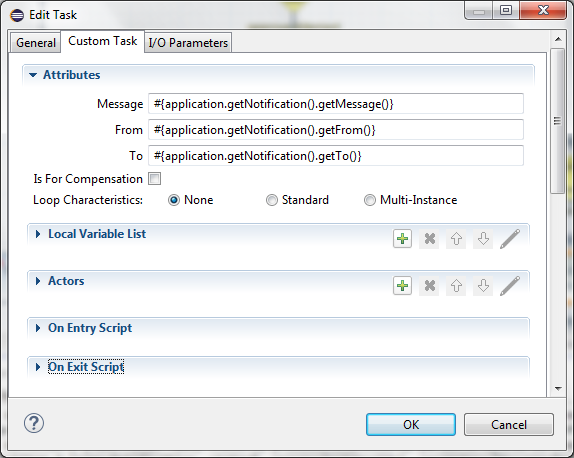
\includegraphics[width=0.8\linewidth]{Bilder/EditCustomTask}
\caption{Eigenschaften der benutzerdefinierten Aufgabe Notification}
\label{fig:EditCustomTask}
\end{figure}


\subsubsection{Der Urlaubsgenehmigungsprozess als BPMN-Diagramm}
Der Workflow ist der elementare Bestandteil unserer Anwendung, in dem die Geschäftsregeln abgebildet werden. Abbildung \ref{fig:Urlaubsantrag} zeigt unseren Urlaubsgenehmigungsprozesses in einem BPMN 2.0 Diagramm.

Unser Workflow startet mit einem Urlaubsantrag (application), der die initialen Daten für den Prozess mitbringt. Der erste Knoten \textit{holiday type} ist ein exklusives Oder und unterscheidet anhand des Urlaubstyps und der gewünschten Anzahl Urlaubstage, ob der Antrag automatisch abgelehnt (rechts, default), automatisch (links) oder manuell (mittig) genehmigt werden muss. Die beiden automatischen Zweige (links und rechts) führen auf direktem Wege durch den jeweiligen Inklusiven Oder-Knoten zum Notification Task und anschließend zum Ende des Workflows.

Der mittlere Zweig der manuellen Genehmigung unterscheidet im nächsten Knoten, dem Exklusiven Oder \textit{board member}, ob der Genehmigungsprozess durch Vorgesetzte und den Leiter der Personalabteilung übersprungen werden darf (links). Dies ist der Fall, wenn die beantragende Person Vorstandsmitglied ist und weniger als 5 Tage Urlaub beantragt. Sollte dies nicht der Fall sein, ist der nächste Knoten das Inklusive Oder \textit{additional HR}. In jedem Fall wird von dort aus der Zweig zur Genehmigung durch den Vorgesetzten (mittig) durchlaufen. Sollten mehr als 20 Tage Urlaub beantragt werden, so wird ebenfalls der Zweig zur Genehmigung durch den Leiter der Personalabteilung fortgesetzt (rechts). Damit diese beiden Zweige parallel abgearbeitet werden können, ist ein Inklusives Oder am Knoten \textit{additional HR} notwendig. Die Genehmigungen werden jeweils durch User Tasks abgebildet.

Im mittleren Zweig wird die Aufgabe dem Vorgesetzten zugewiesen. Dieser User Task \textit{Superior approve} ist um einen Timer erweitert, welcher dafür sorgt, dass die Aufgabe, falls diese nicht in der festgelegten Zeitspanne von 3 Tagen erledigt ist, an den Stellvertreter weitergereicht wird. Dazu verweist der Timer auf den User Task \textit{Co superior approve}. Die Pfade des Vorgesetzten und seines Stellvertreters werden mithilfe des Inklusiven Oders \textit{superior or co} zusammengeführt.

Im rechten Zweig ist der User Task dem Leiter der Personalabteilung zugewiesen. Wichtig ist, dass im Anschluss an die Aufgabe dieser Zweig mit dem mittleren wieder synchronisiert wird. Dazu dienen das Exklusive Oder \textit{additional HR} und das Und \textit{sync superior and HR}. Das Exklusive Oder stellt die Entscheidung dar, ob synchronisiert werden muss, was der Fall ist, wenn zuvor durch eine Beantragung von mehr als 20 Tagen die Personalleitung eingeschaltet wurde. Das Und führt die Synchronisation durch, da der Arbeitsfluss erst fortgesetzt wird, wenn beide Pfade an diesem Punkt angelangt sind.

In dem anschließenden Inklusiven Oder \textit{board member or superior and/or HR} werden die möglichen Pfade des Genehmigungsprozesses durch Vorgesetzte und Personalleitung mit dem des Vorstandsmitglieds zusammengeführt. Das nachfolgende Inklusive Oder \textit{approved/denied} prüft den Status des Antrags. Ist der Antrag an dieser Stelle im Status abgelehnt, führt dies auf direktem Wege (rechts) durch den Inklusiven Oder-Knoten \textit{denied} zum Notification Task und anschließend zum Ende des Workflows. Ist der Status allerdings genehmigt, so wird der Antrag im Folgenden mittels des User Tasks \textit{Advisor hr approve} an den Personalsachbearbeiter gereicht (mittig). Dessen Entscheidung wird im nächsten Knoten, dem Inklusiven Oder \textit{approved or denied}, ausgewertet. Hat der Sachbearbeiter den Antrag abgelehnt (rechts), so wird der Vorgesetzte mit einer gesonderten Notification davon unterrichtet, bevor der Pfad ebenfalls durch den Inklusiven Oder-Knoten \textit{denied} zum Notification Task und anschließend zum Ende des Workflows führt. Hat der Sachbearbeiter hingegen den Antrag genehmigt (links), wird der Pfad mit dem der automatischen Genehmigung im Inklusiven Oder \textit{Auto or Advisor} zusammengeführt, bevor der Workflow nach einer Notification endet. 

\begin{figure}[H]
\centering
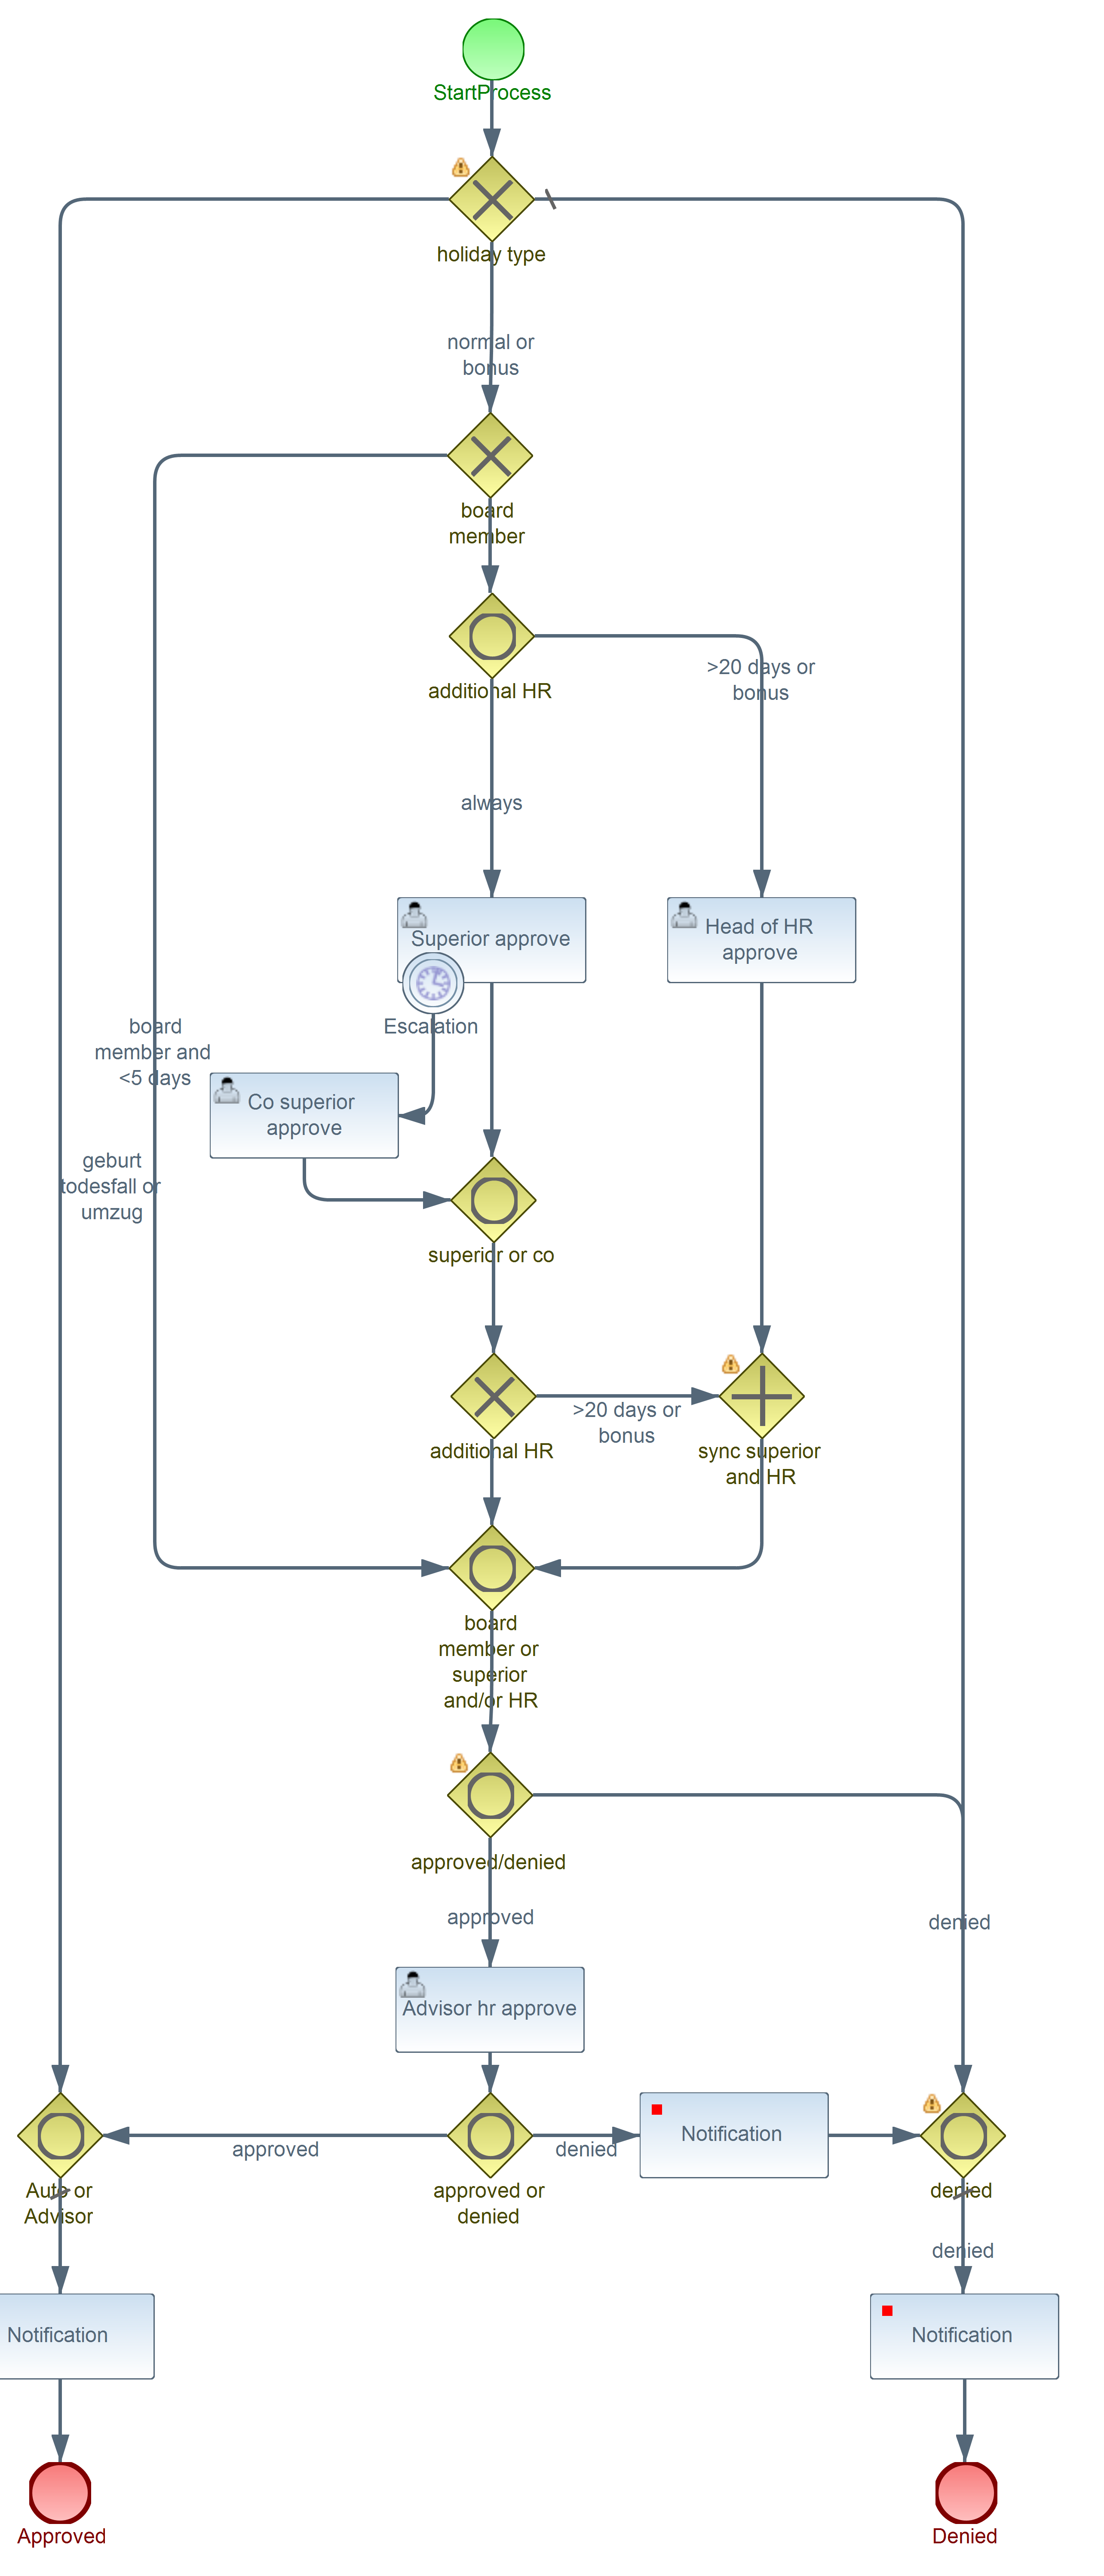
\includegraphics[width=0.75\linewidth]{Bilder/Urlaubsantrag}
\caption{Das BPMN-Diagramm unseres Urlaubsgenehmigungsprozesses}
\label{fig:Urlaubsantrag}
\end{figure}


\subsection{Benutzeroberfläche}
In diesem Abschnitt wollen wir unsere Swing-Benutzeroberfläche, die aus insgesamt drei Dialogen besteht, vorstellen.

\subsubsection{StartDialog}
Über den StartDialog kann der Mitarbeiter einen neuen Urlaubsgenehmigungsprozess starten. Dazu muss er seinen Namen, die Anzahl der Urlaubstage und den Typ seines Urlaubs eingeben. Über die Combobox kann er zwischen den vier Möglichkeiten Normal, Umzug, Geburt- oder Todesfall und Bonus auswählen.

\begin{figure}[H]
	\centering
	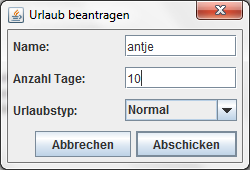
\includegraphics[width=0.4\linewidth]{Bilder/DialogUrlaubBeantragen}
	\caption{Screenshot des StartDialoges}
	\label{fig:DialogUrlaubBeantragen}
\end{figure}

Durch einen Klick auf den Button Abschicken wird ein neuer Prozess gestartet. Alternativ kann der Mitarbeiter den Vorgang auch abbrechen.

\subsubsection{ApproveDialog}
Der ApproveDialog wird verwendet um einen Urlaubsantrag entweder zu genehmigen oder abzulehnen. Da diese Entscheidung in unserem Prozess an mehreren Stellen nötig ist, kommt der Dialog mehrmals zum Einsatz.

Im Titel des Dialogfensters steht die zuständige Person, die für die Abarbeitung dieses Schritte verantwortlich ist. In dem Dialog werden die Informationen, welcher Mitarbeiter wie viele Tage Urlaub eines bestimmten Urlaubstyps beantragt hat, angezeigt.

Abbildung \ref{fig:DialogVorgesetzteGenehmigung} zeigt ein entsprechendes Dialogfenster zur Genehmigung eines Urlaubsantrages am Beispiel von Frau Antje. Als Vorgesetzte von Frau Antje ist Frau Ennel für die Genehmigung des Antrags zuständig.

\begin{figure}[H]
	\centering
	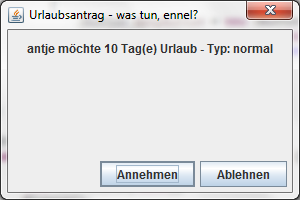
\includegraphics[width=0.5\linewidth]{Bilder/DialogVorgesetzteGenehmigung}
	\caption{Screenshot des ApproveDialogs für die Genehmigung des Vorgesetzten}
	\label{fig:DialogVorgesetzteGenehmigung}
\end{figure}

Über die beiden Buttons Annehmen und Ablehnen kann der Antrag genehmigt bzw. abgelehnt werden.

\subsubsection{NotifierDialog}
Der NotifierDialog wird genutzt um Endanwendern eine Benachrichtigung anzuzeigen. Im Titel des Dialogfensters steht neben dem Empfänger auch der Absender der Nachricht. Innerhalb des Dialogfensters wird die Nachricht dargestellt.

Abbildung \ref{fig:DialogBenachrichtigungGenehmigt} zeigt den entsprechenden Dialog für den genehmigten Urlaubsantrag von Frau Antje. Da der Antrag genehmigt wurde kommt die Nachricht vom System. Im Falle einer Ablehnung wäre der Absender derjenige, der den Antrag abgelehnt hat.

\begin{figure}[H]
\centering
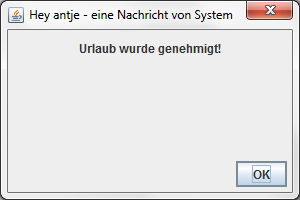
\includegraphics[width=0.5\linewidth]{Bilder/DialogBenachrichtigungGenehmigt}
\caption{Screenshot des NotifierDialogs für einen genehmigten Urlaubsantrag}
\label{fig:DialogBenachrichtigungGenehmigt}
\end{figure}

Über den OK-Button kann die Benachrichtigung geschlossen werden.

\section{Ergebnis}
Für die Überprüfung des Ergebnisses sollten verschiedene Beispielszenarien durchgespielt werden.


Spielen Sie folgende Beispiele durch:


a. Fr. Antje beantragt 10 Tage Urlaub. Ihre Chefin genehmigt den Urlaub, es stehen noch 10
Tage Resturlaub zur Verfügung.


b. Hr. Detuwas möchte 10 Tage Urlaub. Ihm stehen noch 20 Tage Resturlaub zur Verfügung.
Nach drei Tagen hat sein Chef noch nicht reagiert.


c. Hr. Oberboss, der in diesem Jahr noch keinen Urlaub hatte, braucht eine Auszeit und möchte
28 Tage Urlaub, die im Vorstand gerne genehmigt werden.


d. Kurz nach der Rückkehr aus Ihrem Urlaub zieht Frau Antje um und beantragt daher einen Tag
Sonderurlaub.


e. Hr. Auchda (Resturlaub 20 Tage) beantragt 10 Tage Urlaub. Diese werden genehmigt.
\section{Fazit}
Als Ergebnis der Realisierung ist eine prototypische Anwendung entstanden, die den Urlaubsgenehmigungsprozess in einem BPMN-Diagramm abbildet und über eine in Swing realisierte Benutzeroberfläche die Interaktion mit dem Endanwender ermöglicht.

Für die Umsetzung der Aufgabe standen uns das Eclipse-BPMN-Plugin und die KIE Workbench zur Verfügung. Die KIE Workbench hat uns auf den ersten Blick gut gefallen. Durch die Anmeldung unterschiedlicher Benutzer konnte der Ablauf von Prozessen ziemlich realitätsnah simuliert werden. Da der Prozessdesigner jedoch mehrfach fehlerhaftes XML erzeugt hat und damit das BPMN-Diagramm nicht mehr anzeigen konnte haben wir unsere Anwendung letztendlich in Eclipse und dem BPMN Modeler 2.0 Plugin realisiert.

Das Eclipse-Plugin hat uns eine einfache Möglichkeit gegeben den Prozess in einem grafischen Prozessdesigner zu gestalten. Besonders gut gefallen hat uns die Tatsache, dass wir die entsprechenden WorkItemHandler in Java implementieren konnten. So waren wir in der Lage alle externen Abhängigkeiten hinter Schnittstellen zu verstecken und deren Implementierungen einfach auszutauschen. Beispielsweise haben wir zu Beginn unseres Projektes alle Eingaben über die Konsole realisiert und erst später eine Benutzeroberfläche in Swing implementiert.

Die Implementierung der Benutzerschnittstelle musste asynchron erfolgen um beispielsweise Parallelität im Workflow zu ermöglichen. In diesem Zusammenhang ist uns aufgefallen, dass der Logger nur mit einem sequentiellem Prozessablauf umgehen kann. Aufgrund unserer Asynchronizität protokolliert der Logger nur bis zur ersten Benutzerinteraktion.

Insgesamt haben wir für uns festgestellt, dass sich Geschäftsprozesse relativ gut abbilden lassen. Auch die Implementierung eigener "`Custom Tasks"' stellt kein großes Problem da. So ist die Entwicklungsumgebung flexibel und bietet alle nötigen Möglichkeiten einen vollständigen Geschäftsprozess digital abzubilden.

Über das, was wir bisher realisiert haben, hinaus sind weitere Funktionen vorstellbar. Beispielsweise macht eine Persistierung der personenbezogenen Daten Sinn, so dass eine automatische Überprüfung über ausreichend Resturlaubs durchgeführt werden kann. Damit könnte die manuelle Überprüfung in der Personalabteilung entfallen. Außerdem wäre es sinnvoll den Zustand des Workflows zu persistieren, so dass Prozessinstanzen auch nach einem Rechnerausfall weiterhin zur Verfügung stehen. Darüber hinaus ist es denkbar weitere Enterprise Services in den Workflow zu integrieren. Beispielsweise könnte in unserem Prozess die Ermittlung der Vorgesetzten über ein Active-Directory realisiert werden. Des Weiteren könnte die Benachrichtigung der Mitarbeiter über einen E-Mail-Dienst erfolgen. Zusätzliche Erweiterungen oder Anpassungen sind selbstverständlich vorstellbar.

Unsere prototypische Anwendung erfüllt die grundlegenden Anforderungen an einen Urlaubsgenehmigungsprozess, die flexibel erweitert und angepasst werden kann und uns einen guten Einblick in das Thema Business Process Modelling gewährt hat.


\appendix
\section{Anhang}

Hier kommt der Anhang.


\newpage
%\printbibliography

\end{document}